%==============================================================================
% Šablona prezentace/Presentation template
% Autoři / Authors: Zdeněk Vašíček, Aleš Smrčka, Jaroslav Dytrych, Jana Stopková, Kristýna Zaklová, Adam Herout
% Kontakt pro dotazy a připomínky: sablona@fit.vutbr.cz
% Contact for questions and comments: sablona@fit.vutbr.cz
%==============================================================================

\documentclass[]{fitthesispresn}

\usepackage[czech, ruled, linesnumbered]{algorithm2e}

% Nastavení informací pro úvodní stránku / Setting information for the title page
%---------------------------------------------------------------------------
\projectinfo{
  date=\today, % Datum - je vhodné vepsat datum obhajoby (natvrdo), ne datum kompilace slajdů / Date - it is advisable to write the date of the defense (hard), not the date of the slide compilation        
  title={Hashovací tabulka}, % Název prezentace / Presentation title (The whole title of the presented work suitably divided into lines that are optically balanced)
  title.footer={Hashovací tabulka}, % Název prezentace - text zobrazovaný vedle čísla slajdu / Presentation title - displayed next to the slide number (The full title of the presented work, it may be suitably abbreviated to fit the footer)
  author.name={Lukáš},  % Jméno autora / Author name
  author.surname={Pšeja}, % Příjmení autora / Author surname
  author.title.first={} % Tituly před jménem autora (jsou-li jaké) / Author's titles before the name (if there are any)
}

% Struktura prezentace / Presentation structure
%---------------------------------------------------------------------------

\begin{document}
    \frame[plain]{\titlepage} % Úvodní stránka / Title page

    \begin{frame}
        \frametitle{Motivace}
        \begin{itemize}
            \item Hashovací tabulka nám dovoluje rychle vyhledávat a ukládat data
            \item Využívá se v databázích, překladačích, operačních systémech, atd.
            \item \emph{Výhody}\,--\,rychlost, jednoduchost, efektivita
            \item \emph{Nevýhody}\,--\,kolize, paměťová náročnost
        \end{itemize}
    \end{frame}

    \begin{frame}
        \frametitle{Co je to hashovací tabulka?}
        \begin{columns}
            \column{0.4\textwidth}
            \begin{itemize}
                \item Hashovací tabulka je datová struktura
                \item Je implementována pomocí asociativního pole
                \item Ukládá data ve formě \emph{klíč-hodnota}
                \item Umožňuje rychlé \emph{vyhledávání}, \emph{vkládání} a \emph{mazání} prvků pomocí použití \emph{hashovací funkce}
            \end{itemize}
            \column{0.6\textwidth}
            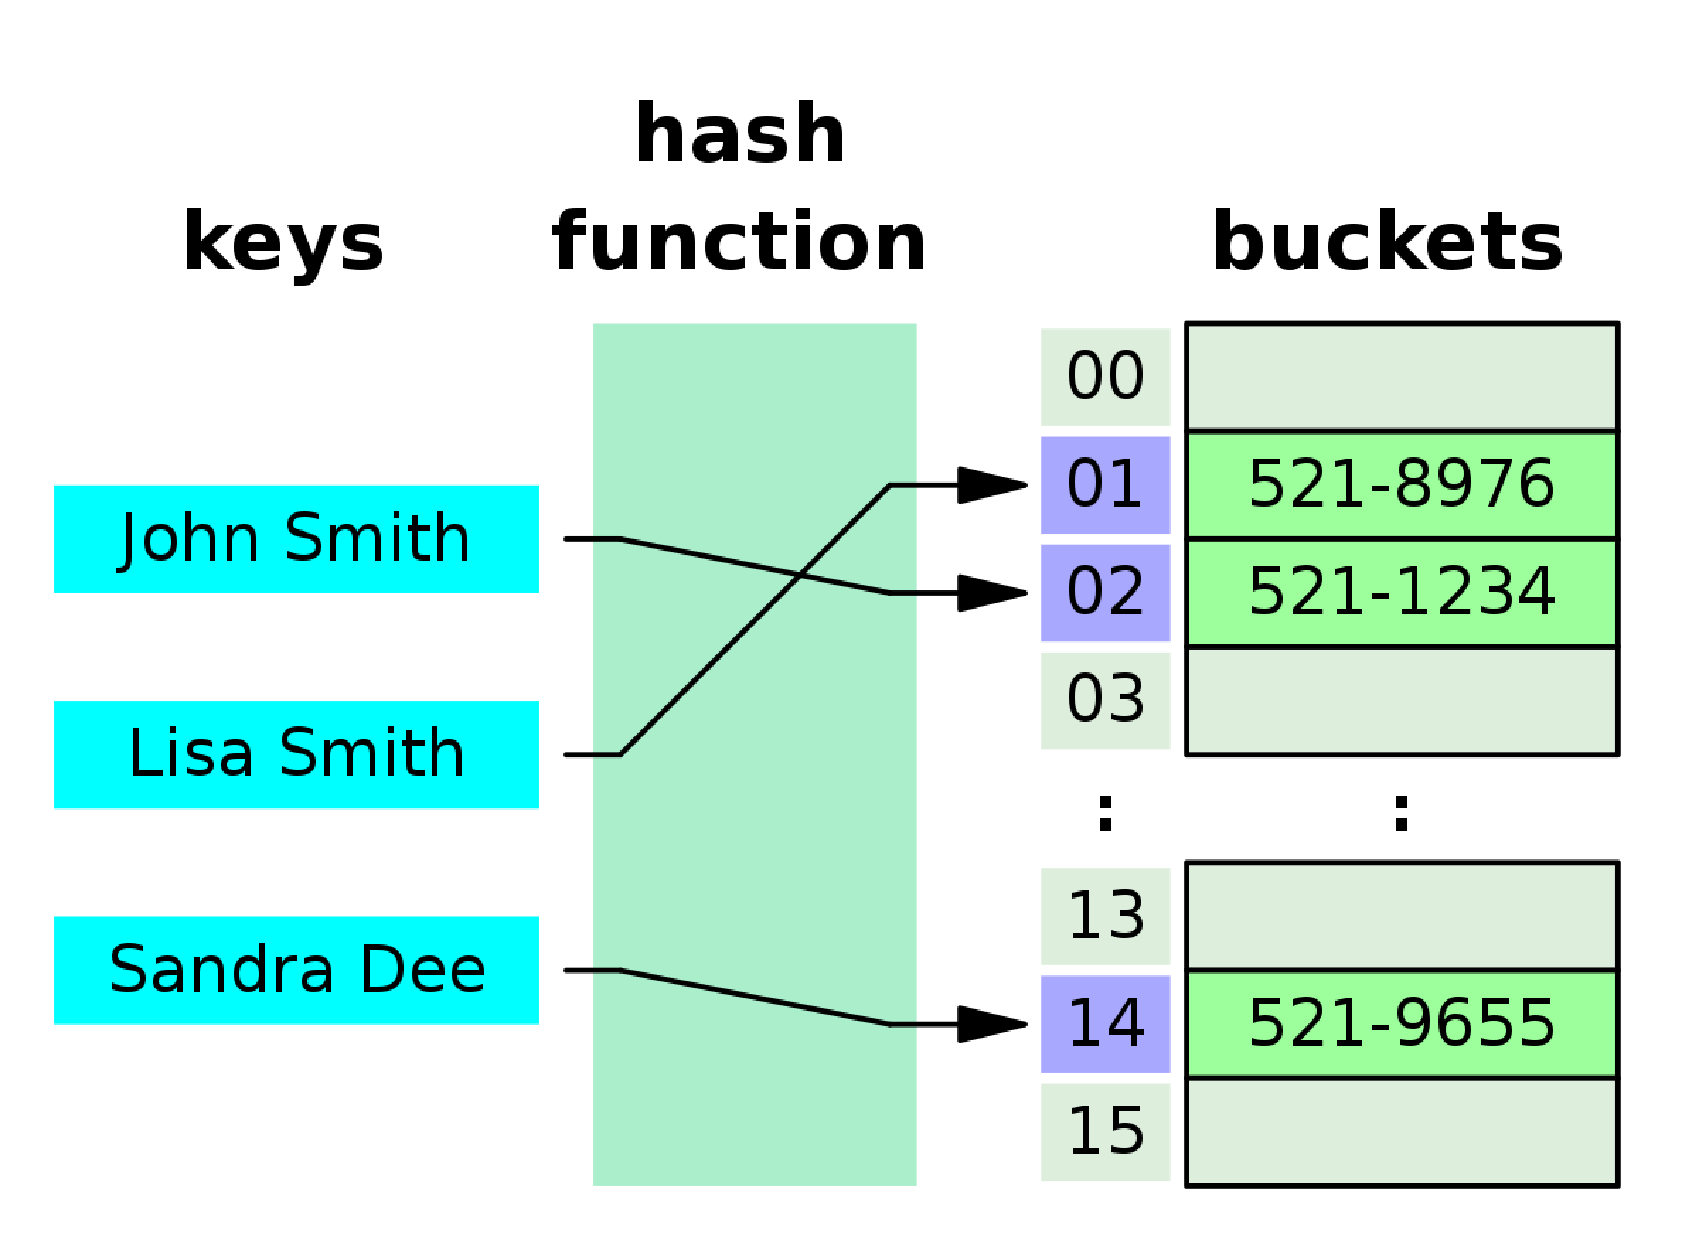
\includegraphics[width=\textwidth]{img/hash_table.pdf} % wikipedie - hash table
        \end{columns}
    \end{frame}

    \begin{frame}
        \frametitle{Struktura hashovací tabulky}
        \begin{columns}
            \column{0.4\textwidth}
            \begin{itemize}
                \item \emph{Počet záznamů} je počet prvků klíč-hodnota v hashovací tabulce, v obrázku 3
                \item \emph{Počet ukazatelů v poli ukazatelů} určuje počet ukazatelů v poli ukazatelů, v obrázku 4
                \item \emph{Pole ukazatelů} je vždy jedno
            \end{itemize}
            Inspirováno hashovací tabulkou z předmětu IJC
            \column{0.6\textwidth}
            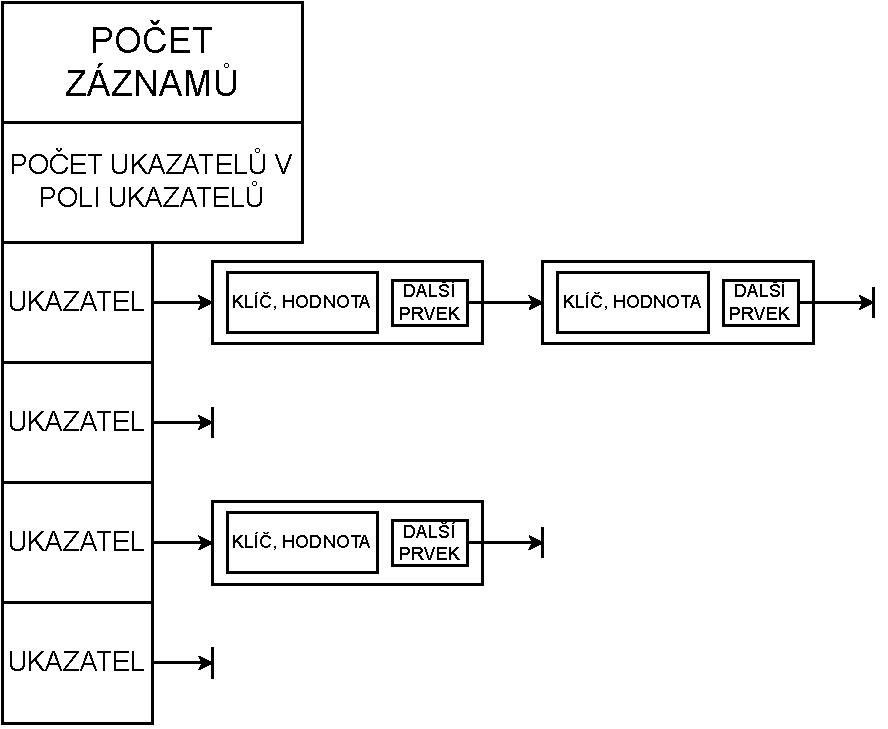
\includegraphics[width=\textwidth]{img/hash_table_ijc.pdf}
        \end{columns}
    \end{frame}

    \begin{frame}
        \frametitle{Základní operace s hashovací tabulkou 1/2}
            Pro následující ukázky uvažujme \emph{inicializovanou} hashovací tabulku pro počítání slov v textu.

            \begin{algorithm}[H]
                \caption{Vložení klíče \texttt{key} do tabulky} \label{alg:insert}
                \SetKwInOut{Input}{Input}
                \SetKwInOut{Output}{Output}
                \Input{Hashovací tabulka \texttt{ht}, klíč \texttt{key}}
                \Output{\texttt{0} při úspěchu, \texttt{1} při chybě}
                \BlankLine
                \SetAlgoLined
                \SetKwFunction{Insert}{Insert}
                \Insert{\texttt{ht}, \texttt{key}, \texttt{value}}
            \end{algorithm}
    \end{frame}








    \begin{frame}
        \frametitle{Cíle práce}
        \begin{columns}
            \column{0.4\textwidth}
            \begin{itemize}
                \item \emph{Vstup}
                \item \emph{Výstup}
                \item Žádoucí \emph{vlastnosti}
                \item Využití \& aplikace
            \end{itemize}

            \column{0.6\textwidth}
            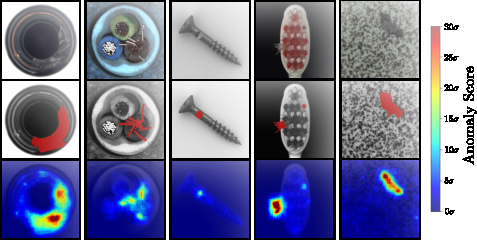
\includegraphics[width=\textwidth]{img/template-Goal.pdf}
        \end{columns}
    \end{frame}

    \begin{frame}
        \frametitle{Podstatné informace o řešení}
        \centering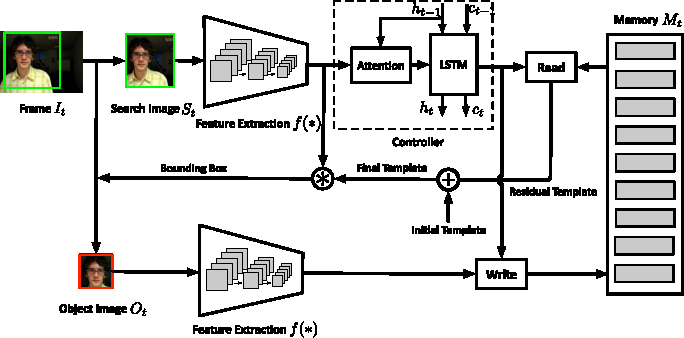
\includegraphics[width=0.8\textwidth]{img/template-Schema.pdf}
        \begin{equation}
            \mathbf{a}_t = \sum_{i=1}^{L}\alpha_{t,i}\mathbf{f}_{t,i}^{*}
        \end{equation}
        kde $\alpha_{t,i}$ počítá \emph{softmax}:
        \begin{align}
            \alpha_{t,i} & = \frac{\exp(r_{t,i})}{\sum_{k=1}{L}\exp(r_{t,k})}
            \\
            r_{t,i}      & = W^a \tanh\left( W^h \mathbf{h}_{t-1} + W^f\mathbf{f}_{t,i}^{*} + b \right)
        \end{align}
    \end{frame}

    \begin{frame}\frametitle{Podstatné informace o řešení}
        \makebox[\linewidth]{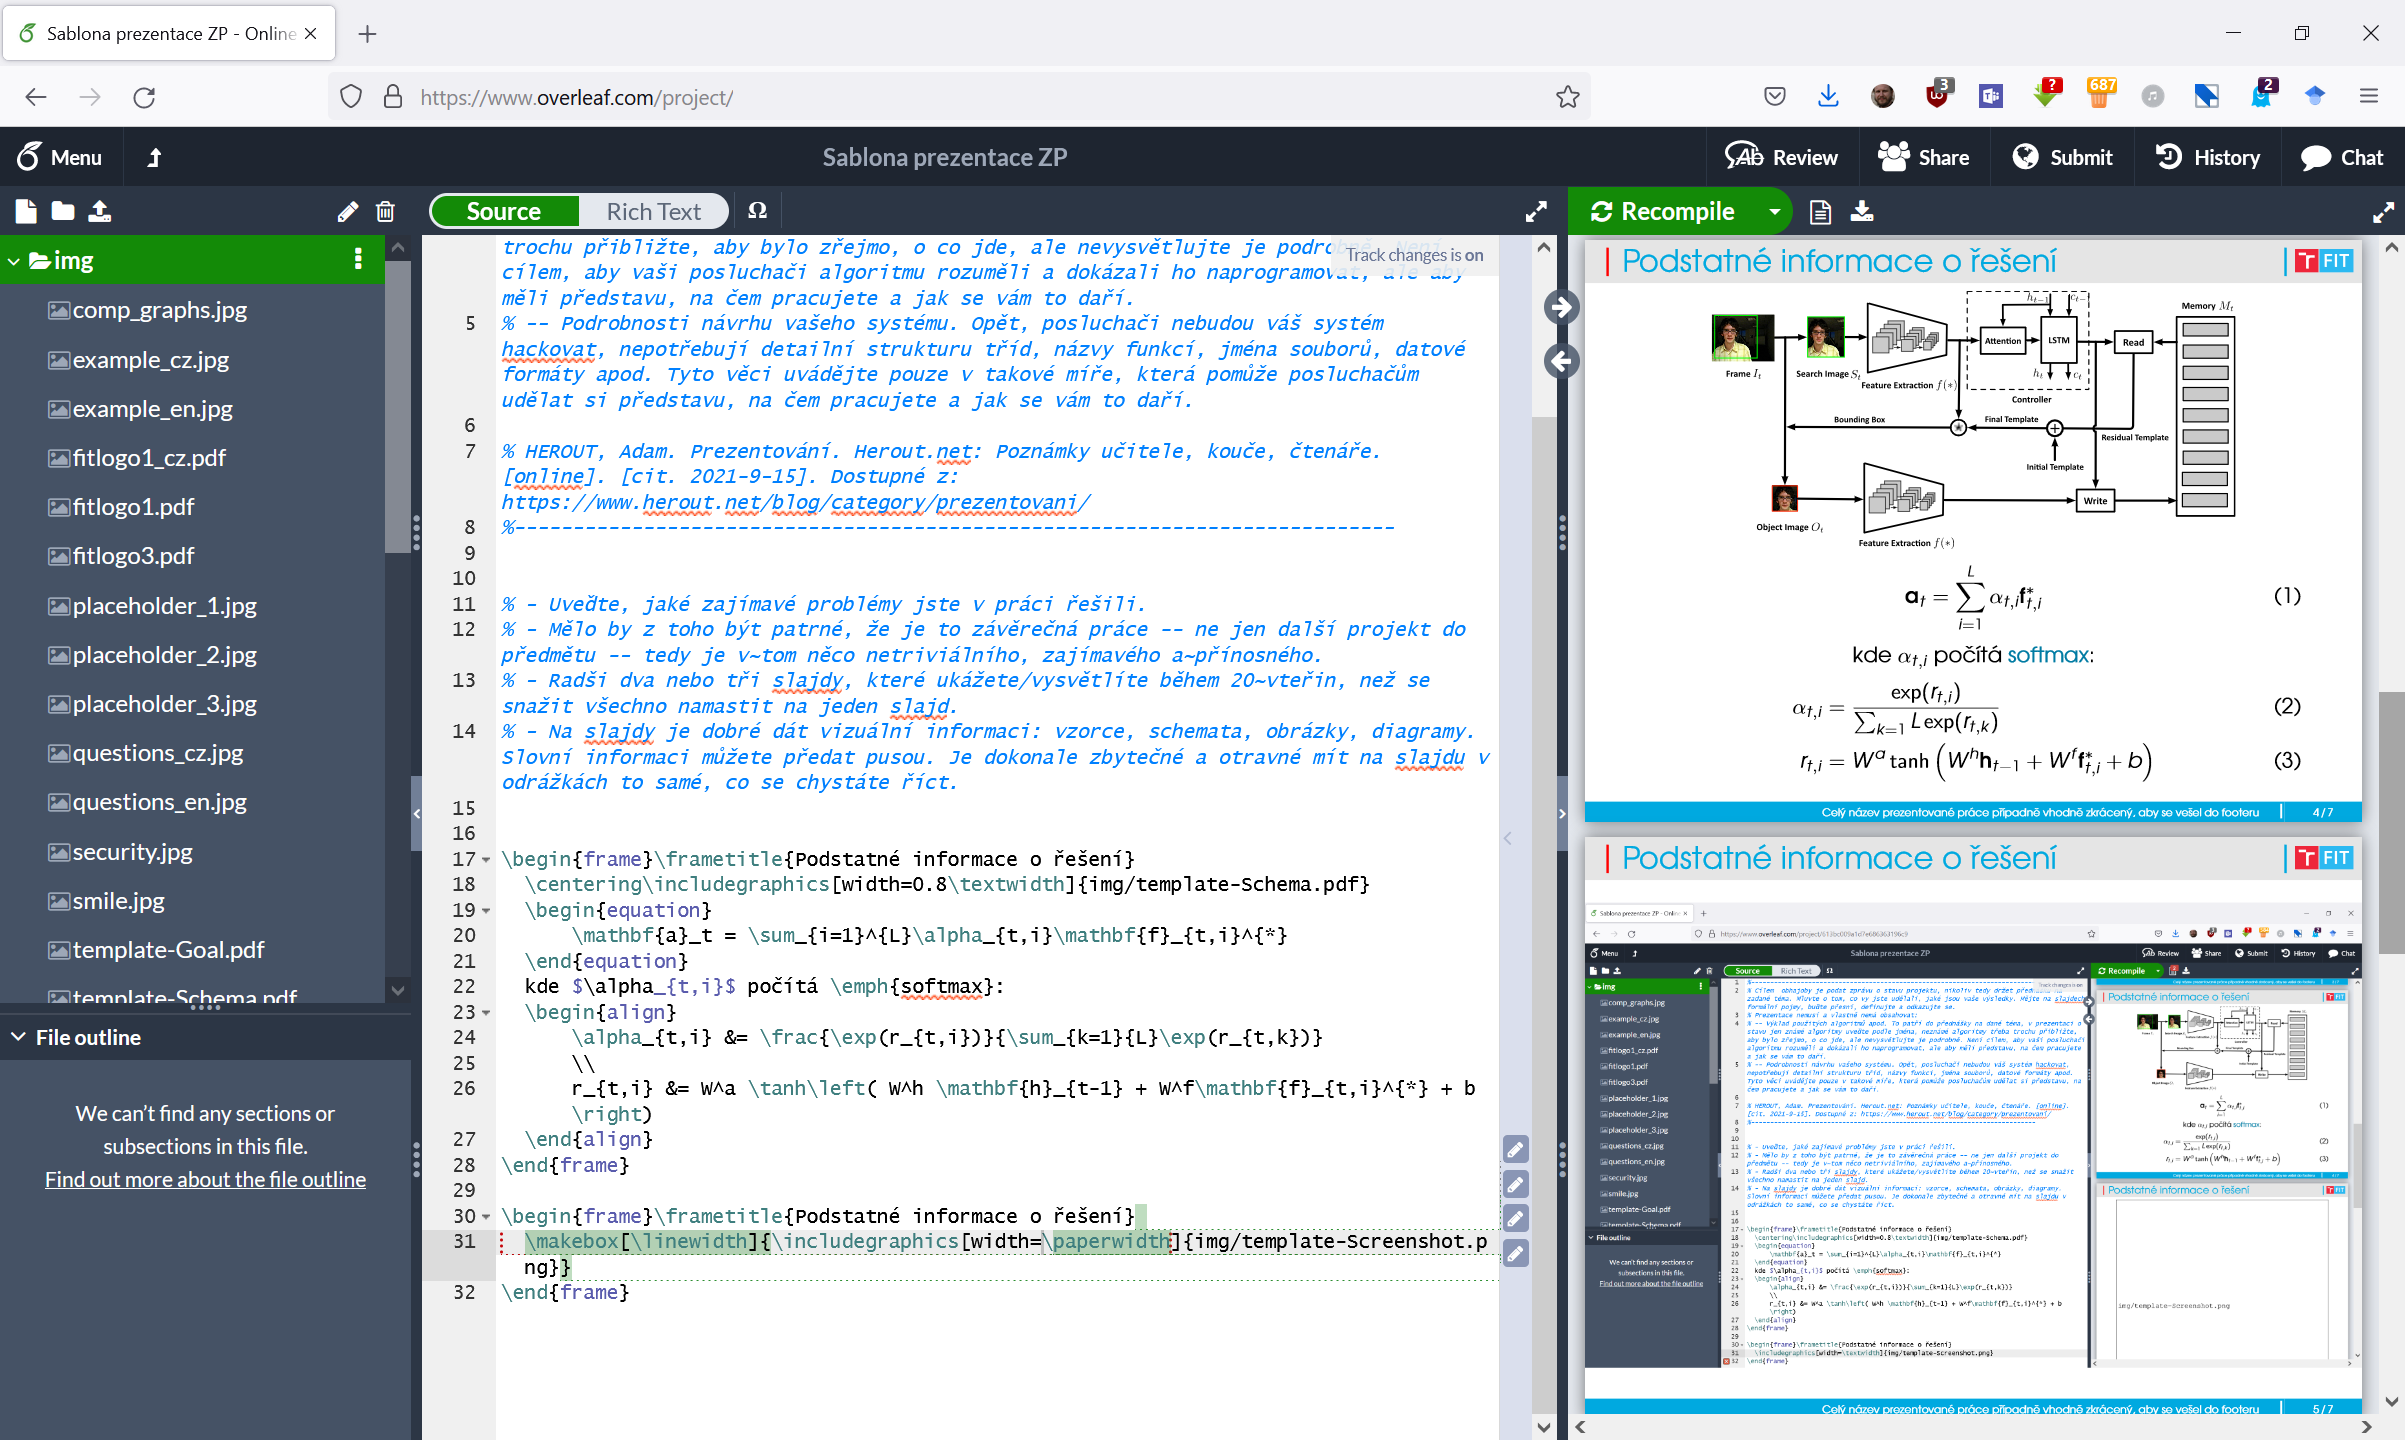
\includegraphics[width=\paperwidth]{img/template-Screenshot.png}}
    \end{frame}

    \begin{frame}
        \frametitle{Výsledky práce}
        \begin{columns}
            \column{0.4\textwidth}
            \begin{itemize}
                \item Co se \emph{podařilo}
                \item Vytvořená datová sada: \emph{105\,k} záznamů
                \item Úspěšnost: \emph{103\,\%}
            \end{itemize}

            \column{0.6\textwidth}
            \centering
            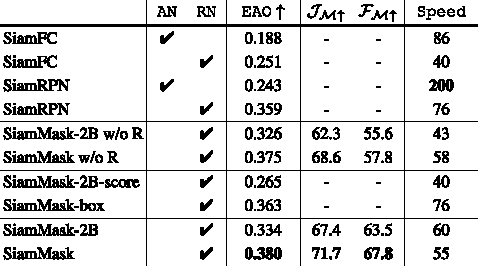
\includegraphics[width=0.8\textwidth]{img/template-ResultsTable.pdf}

            \bigskip
            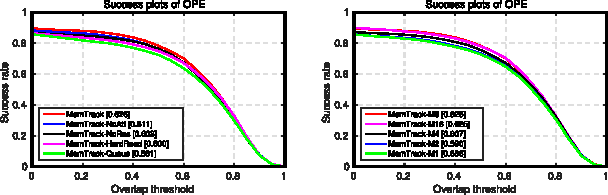
\includegraphics[width=\textwidth]{img/template-ResultsPlot.pdf}

        \end{columns}
    \end{frame}

    \begin{frame}
        \frametitle{Děkuji za pozornost!}
        \centering
        \makebox[\textwidth]{
            \begin{tikzpicture}
                \node (screenshot)
                {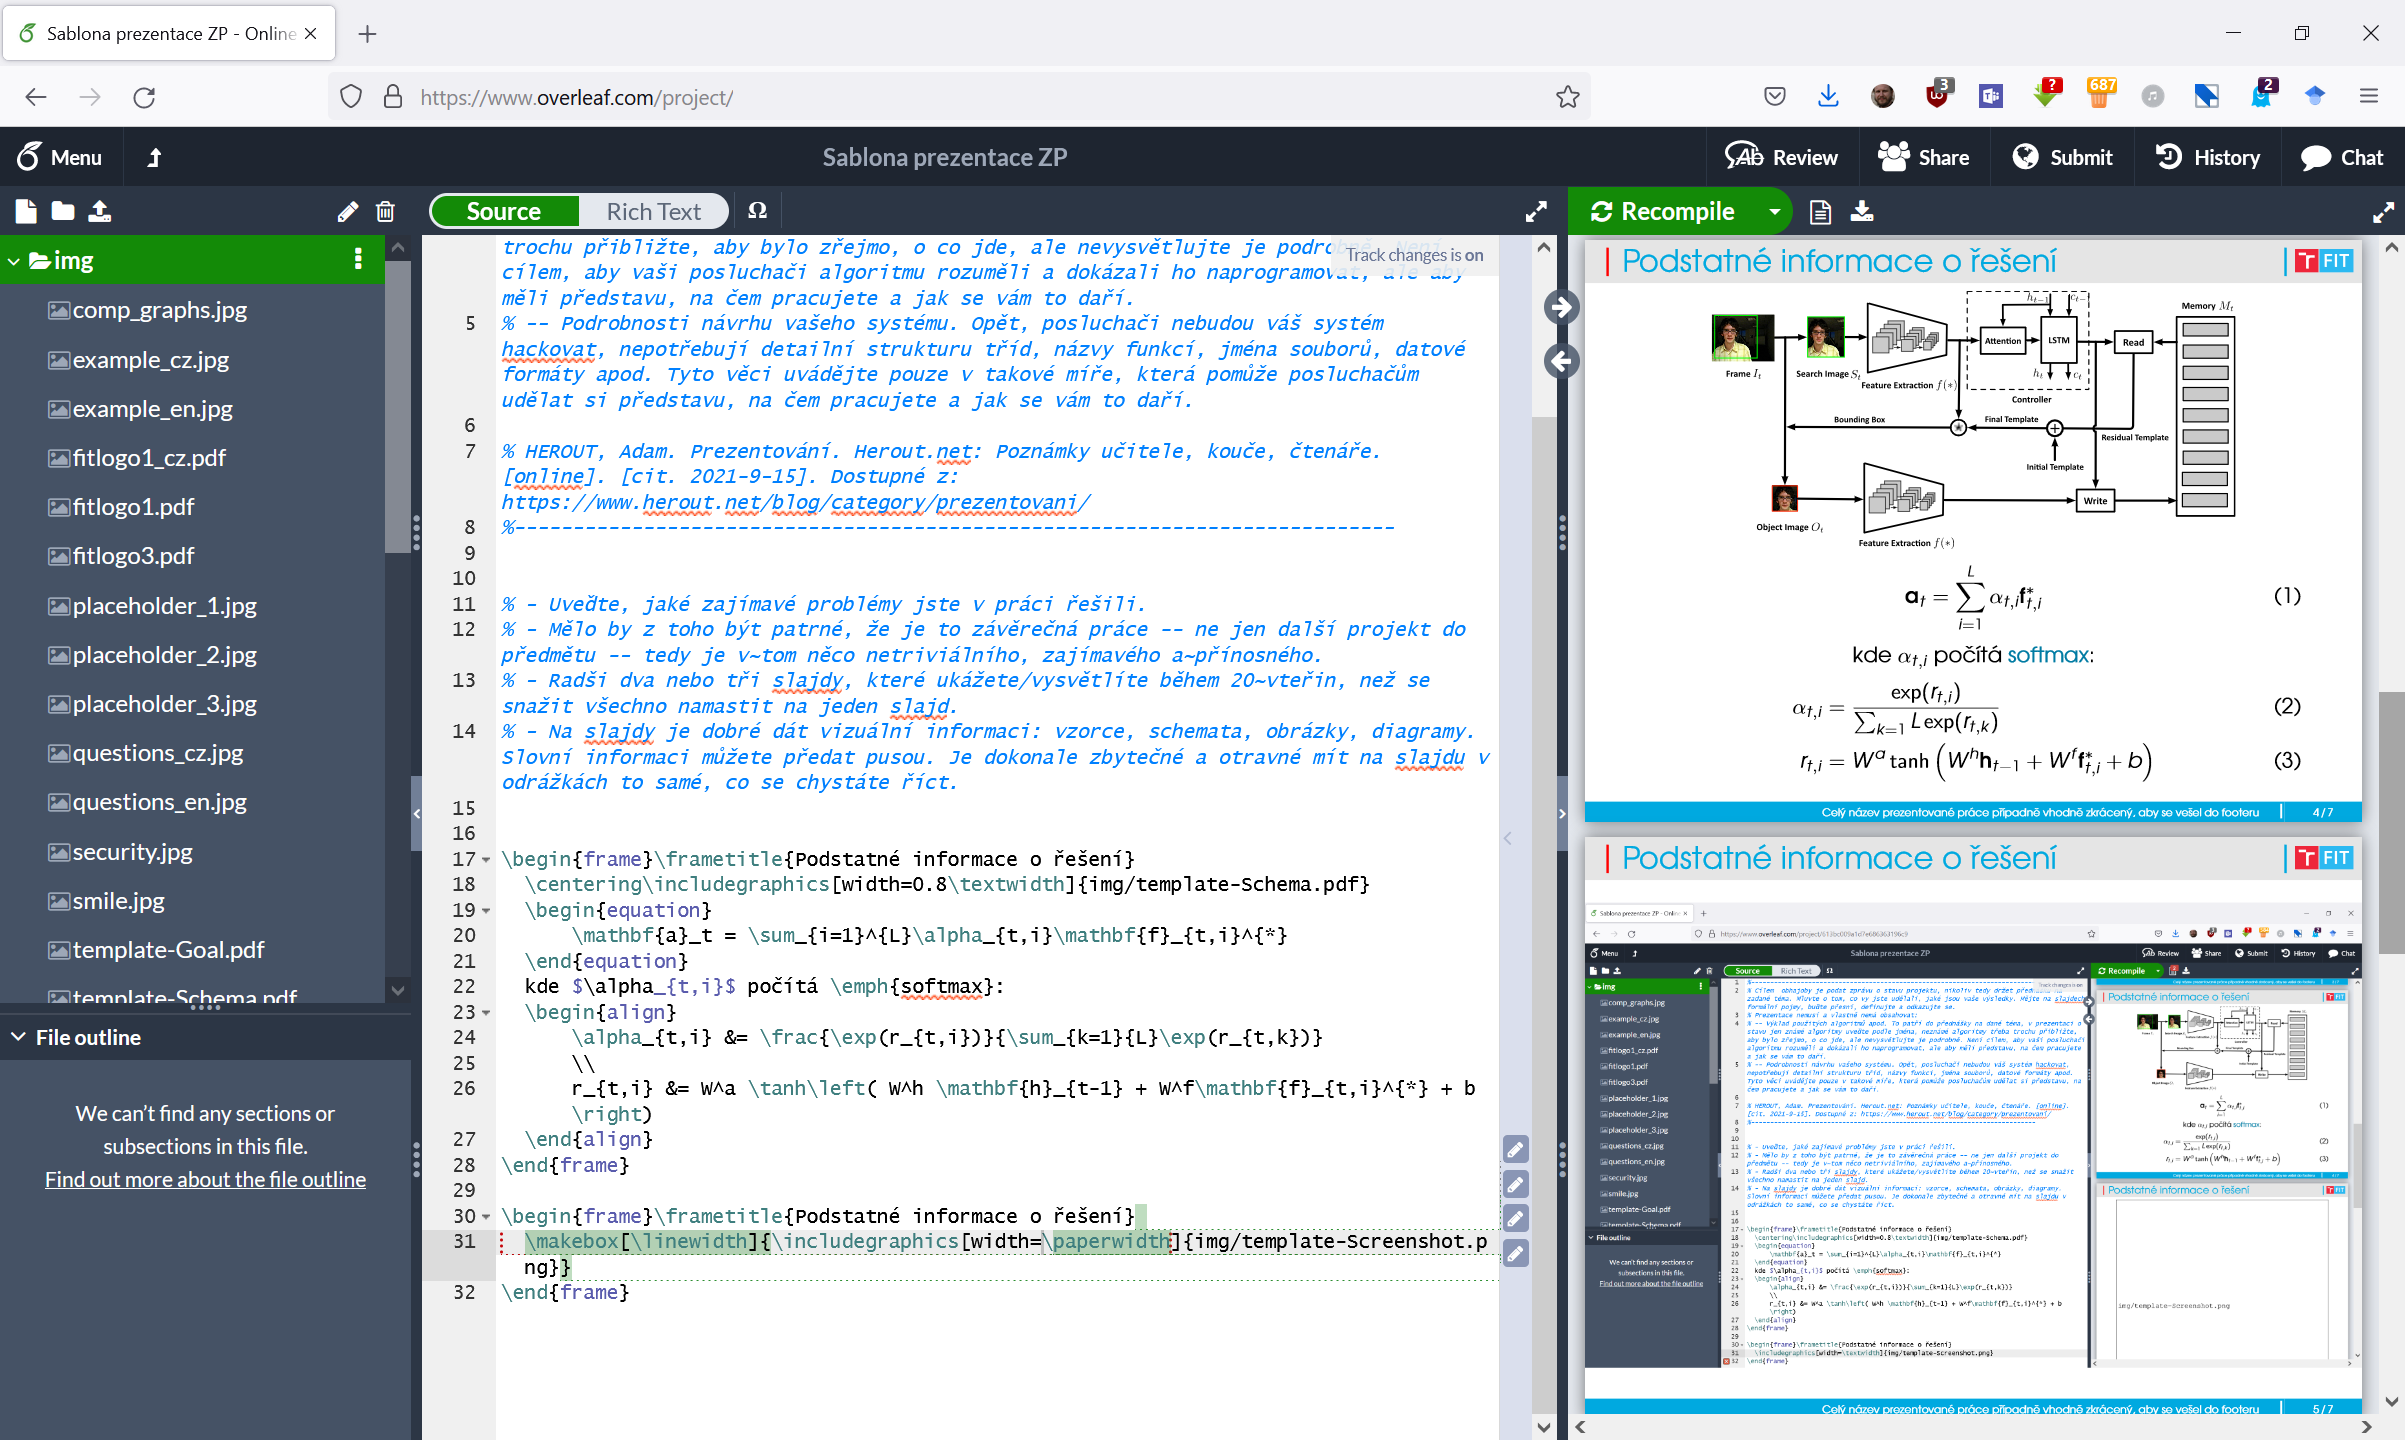
\includegraphics[width=0.6\paperwidth]{img/template-Screenshot.png}};
                \node (schema) at (screenshot.south east) [xshift=5em] [yshift=2.5ex]
                {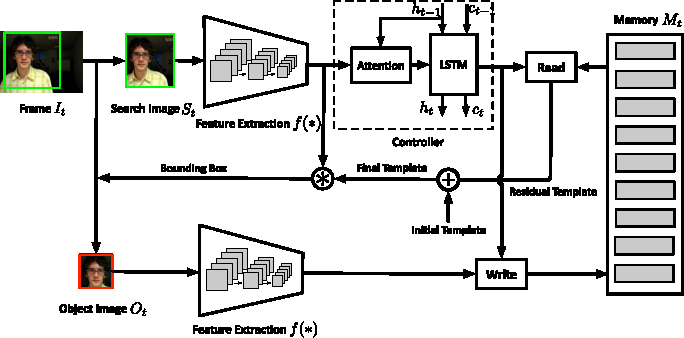
\includegraphics[width=0.45\paperwidth]{img/template-Schema.pdf}};
                \node (goal) at (screenshot.north east) [xshift=4em] [yshift=2ex]
                {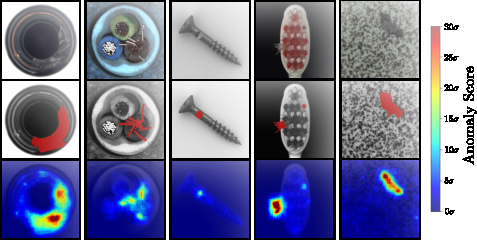
\includegraphics[width=0.5\paperwidth]{img/template-Goal.pdf}};
            \end{tikzpicture}
        }
    \end{frame}
\end{document}
